\chapter{The Visualization Pipeline}
\label{chap:visualization_pipeline}

\begin{figure}[ht]
	\hfill
	\begin{minipage}{0.5\textwidth}
		\centering
		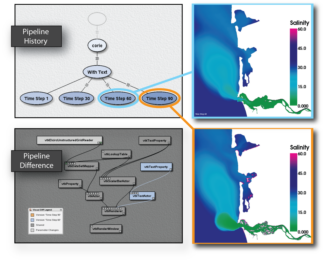
\includegraphics{VTKTextbook-38}\\
		\caption*{\texttt{The VisTrails multi-view visualization system.
				VisTrials enables interactive creation of visualization pipelines, maintaining the history of their evolution, optimizing their execution and allowing multiple pipelines to be compared in a spreadsheet-style layout.
				Image courtesy of SCI Institute University of Utah.}}
	\end{minipage}
\end{figure}

\firstletter{I}n the previous chapter we created graphical images using simple mathematical models for lighting, viewing, and geometry.
The lighting model included ambient, diffuse, and specular effects.
Viewing included the effects of perspective and projection.
Geometry was defined as a static collection of graphics primitives such as points and polygons.
In order to describe the process of visualization we need to extend our understanding of geometry to include more complex forms.
We will see that the visualization process transforms data into graphics primitives.
This chapter examines the process of data transformation and develops a model of data flow for visualization systems.

\section {Overview}
Visualization transforms data into images that efficiently and accurately convey information about the data.
Thus, visualization addresses the issues of \emph{transformation} and \emph{representation}.

Transformation is the process of converting data from its original form into graphics primitives, and eventually into computer images. This is our working definition of the visualization process. An example of such a transformation is the process of extracting stock prices and creating an *x-y* plot depicting stock price as a function of time.

Representation includes both the internal data structures used to depict the data and the graphics primitives used to display the data. For example, an array of stock prices and an array of times are the computational representation of the data, while the \emph{x-y} plot is the graphical representation. Visualization transforms a computational form into a graphical form.

From an object-oriented viewpoint, transformations are processes in the functional model, while representations are the objects in the object model. Therefore, we characterize the visualization model with both functional models and object models.

\subsection{A Data Visualization Example}

A simple mathematical function for a quadric will clarify these
concepts. The function

\begin{equation}\label{eq:4.1}
F(x,y,z) = a_0x^2 + a_1y^2 + a_2z^2 + a_3xy + a_4yz + a_5xz + a_6x + a_7y + a_8z + a9
\end{equation}
\myequations{A quadric function. }

is the mathematical representation of a quadric. Figure \ref{fig:Figure4-1a} shows a visualization of Equation \ref{eq:4.1} in the region $-1 \leqslant x, y, z \leqslant 1$. The visualization process is as follows. We sample the data on a regular grid at a resolution of $50 x 50 x 50$. Three
different visualization techniques are then used.
On the left, we generate 3D surfaces corresponding to the function $F(x,y,z) = c$ where $c$ is an arbitrary constant (i.e., the isosurface
value).
In the center, we show three different planes that cut through the data and are colored by function value.
On the right we show the same three planes that have been contoured with constant valued lines.
Around each we place a wireframe outline.

\subsection{The Functional Model}

The functional model in Figure \ref{fig:Figure4-1b} illustrates the steps to create the visualization.
The oval blocks indicate operations (processes) we performed on the data, and the rectangular blocks represent data stores (objects) that represent and provide access to data.
Arrows indicate the direction of data movement.
Arrows that point into a block are inputs; data flowing out of a block indicate outputs.
The blocks also may have local parameters that serve as additional input.
Processes that create data with no input are called data \emph{source} objects, or simply sources. Processes that consume data with no output are called \emph{sinks} (the are also called \emph{mappers} because these processes map data to a final image or output).
Processes with both an input and an output are called \emph{filters}.

The functional model shows how data flows through the system.
It also describes the depen-dency of the various parts upon one another.
For any given process to execute correctly, all the inputs must be up to date.
This suggests that functional models require a synchronization mechanism to insure that the correct output will be generated.

\subsection{The Visualization Model}

In the examples that follow we will frequently use a simplified representation of the functional model to describe visualization processes (Figure \ref{fig:Figure4-1c}).
We will not explicitly distinguish between sources, sinks, data stores, and process objects.
Sources and sinks are implied based on the number of inputs or outputs.
Sources will be process objects with no input. Sinks will be process
objects with no output.
Filters will be process objects with at least one input and one output.
Intermediate data stores will not be represented.
Instead we will assume that they exist as necessary to support the data flow.
Thus, as Figure \ref{fig:Figure4-1c} shows, the \emph{Lines} data store that the \emph{Outline} object generates (Figure \ref{fig:Figure4-1b}) are combined into the single object \emph{Outline}. We use oval shapes to represent objects in the visualization model.

\begin{figure}[htb]
	\begin{subfigure}[h]{0.80\linewidth}
		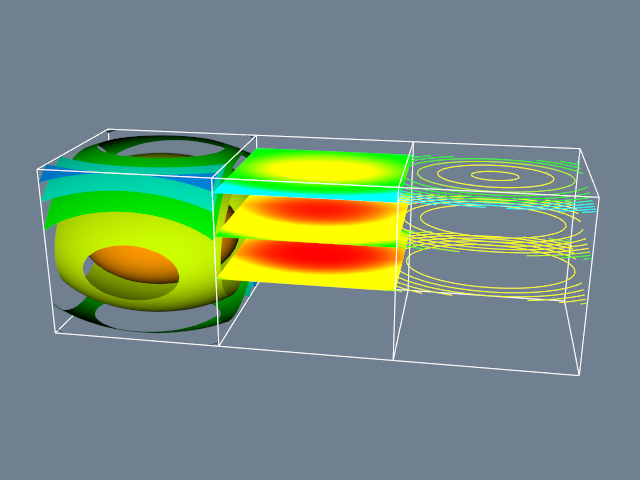
\includegraphics[width=\linewidth]{Figure4-1a}
		\caption{Quadric visualization. (\href{https://lorensen.github.io/VTKExamples/site/Cxx/Visualization/QuadricVisualization/}{QuadricVisualization.cxx} or \href{https://lorensen.github.io/VTKExamples/site/Python/Visualization/QuadricVisualization/}{QuadricVisualization.py})}
		\label{fig:Figure4-1a}
	\end{subfigure}
	\hfill
	\begin{subfigure}[h]{0.80\linewidth}
		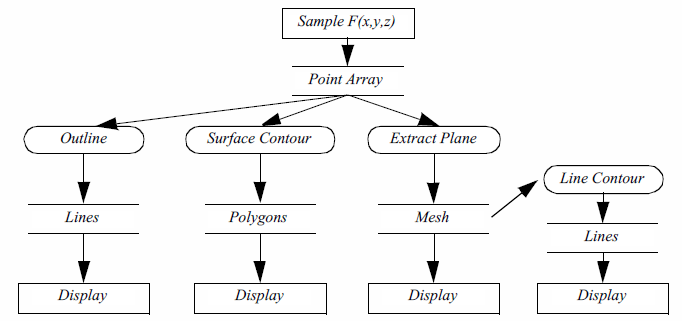
\includegraphics[width=\linewidth]{Figure4-1b}
		\caption{Functional model.}\label{fig:Figure4-1b}
	\end{subfigure}%
	\hfill
	\begin{subfigure}[h]{0.80\linewidth}
		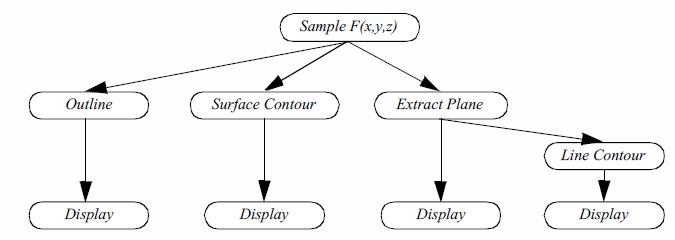
\includegraphics[width=\linewidth]{Figure4-1c}
		\caption{Visualization network.}\label{fig:Figure4-1c}
	\end{subfigure}
	\caption{Visualizing a quadric function $F(x,y,z) = c$.}\label{fig:Figure4-1}
\end{figure}
